\section{Архитектура} \label{architecture}

\subsection{Общая архитектура}

Архитектура продиктована вышеперечисленными требованиями к библиотеке: прозрачный интерфейс с поддержкой подключения своего алгоритма сжатия, эффективная индексация логических блоков, многофайловость.

\begin{itemize}
    \item Интерфейс библиотеки буквально состоит из стандартных операций \texttt{open/close/read/write/seek/tell}, и с точки зрения пользователя нет практически никакой разницы между \texttt{compio} и \texttt{stdio} (кроме конфигурации и понятия многофайловости).
    \item Файл делится на логические блоки, каждый из который сжимается независимо, и для их эффективной индексации используется \textit{B-дерево} (обоснование данного выбора описано в разделе \ref{btree}). Таким образом, для чтения/модификации какого-то участка данных необходимо распаковать только те блоки, которые непосредственно касаются этого участка.
    \item Алгоритм сжатия полностью вынесен из логики библиотеки в качестве абстракции, и от него требуются только 3 функции: \texttt{compress}, \texttt{decompress} и \texttt{get\_buf\_size}, которые пользователь может реализовать сам для любого алгоритма сжатия.
    \item Для того, чтобы хранить все нужные структуры в одном файле был реализован аллокатор блоков внутри файла\footnote{Низкоуровневый аллокатор блоков внутри файла-контейнера разработан Д.\,В.~Корбелайнен. Детали его реализации выходят за рамки настоящей работы.}, который позволяет хранить в одном файле множество независимых структур (заголовок, сжатые блоки разных файлов, узлы B-дерева).
    \item Для индексации внутри B-дерева используется составной ключ из хэша имени логического файла и позиции внутри него, что позволяет хранить все логические блоки в одном B-дереве, за счёт чего достигается многофайловость. Такое решение было выбрано в пользу двух аргументов: снижается нагрузка на низлежащую файловую систему (в случае когда требуется работать с множеством логических файлов), а так же упрощается перенос архива с одной машины на другую.
\end{itemize}

\subsection{Файл-контейнер}

\begin{figure}[htbp]
\centering

\begin{tikzpicture}[
    every node/.style={font=\small},
    table/.style={draw, inner sep=2pt, align=left},
    arrow/.style={-{Stealth[length=3mm]}, thick, black}
]

\node[table, fill=yellow!20, anchor=north west] (header) at (0,0) {
    \begin{tabular}{l}
        \textbf{Header} \\
        \hline
        magic\_number : int32\_t \\
        \hline
        index\_root : uint64\_t \\
        \hline
        file\_size : uint64\_t \\
        \hline
        block\_size : uint32\_t \\
        \hline
        b\_tree\_degree : uint32\_t \\
        \hline
        files\_table\_addr : uint64\_t \\
        \hline
        allocator\_state\_offset : uint64\_t \\
        \hline
        compression\_type : uint32\_t \\
        \hline
        checksum : uint8\_t[32]
    \end{tabular}
};

\node[table, fill=orange!20, right=2cm of header.north east, anchor=north west] (ftable) {
    \begin{tabular}{l}
        \textbf{Files Table} \\
        \hline
        n\_files : uint64\_t \\
        \hline
        max\_files : uint32\_t \\
        \hline
        files : struct file[\,] \\
        \hline
        \qquad name : uint8\_t[ ] \\
        \hline
        \qquad size : uint64\_t
    \end{tabular}
};

\node[table, fill=blue!10, below=0.8cm of header.south west, anchor=north west] (rootnode) {
    \begin{tabular}{l}
        \textbf{B‑Tree Node (Root)} \\
        \hline
        is\_leaf : uint8\_t \\
        \hline
        num\_keys : uint32\_t \\
        \hline
        tree\_degree : int32\_t \\
        \hline
        keys : tree\_key[\,] \\
        \hline
        values : tree\_val[\,] \\
        \hline
        children : uint64\_t[\,] \\
        \hline
        key\_additions : int64\_t[\,]
    \end{tabular}
};

\node[table, fill=green!10, below=0.6cm of ftable.south east, anchor=north east] (blockA) {
    \begin{tabular}{l}
        \textbf{Storage Block} \\
        \hline
        signature : uint8\_t \\
        \hline
        is\_compressed : uint8\_t \\
        \hline
        size : uint64\_t \\
        \hline
        original\_size : uint64\_t \\
        \hline
        checksum : uint32\_t \\
        \hline
        data : uint8\_t[\,]
    \end{tabular}
};

\node[table, fill=green!10, below=0.3cm of blockA.south east, anchor=north east] (blockB) {
    \begin{tabular}{l}
        \textbf{Storage Block} \\
        \hline
        \ldots
    \end{tabular}
};

\node[table, fill=green!10, below=0.6cm of blockB.south east, anchor=north east] (blockC) {
    \begin{tabular}{l}
        \textbf{Storage Block} \\
        \hline
        \ldots
    \end{tabular}
};

\node[table, fill=blue!10, left=0.6cm of blockC.south west, anchor=south east] (childnode) {
    \begin{tabular}{l}
        \textbf{B‑Tree Node} \\
        \hline
        \ldots
    \end{tabular}
};

\draw[arrow] ([yshift=-3.4cm] header.north east) to[out=0, in=180, looseness=0.5] ([yshift=-0.3cm] ftable.north west);

\draw[arrow] ([yshift=-1.4cm] header.north east) to[out=0, in=0, looseness=0.8] ([yshift=-0.3cm] rootnode.north east);

\draw[arrow] ([yshift=-3.0cm] rootnode.north east) to[out=0, in=180, looseness=0.5] ([yshift=-0.3cm] blockA.north west);
\draw[arrow] ([yshift=-3.0cm] rootnode.north east) to[out=0, in=180, looseness=0.5] ([yshift=-0.3cm] blockB.north west);

\draw[arrow] ([yshift=-3.6cm] rootnode.north east) to ([yshift=-0.3cm] childnode.north west);

\draw[arrow] ([yshift=-0.3cm] childnode.east) to[out=0, in=220, looseness=1.2] ([yshift=-0.3cm] blockC.north west);

\end{tikzpicture}

\caption{Структуры внутри файла-контейнера и связи между ними.}
\label{fig:container}
\end{figure}

\begin{figure}[htbp]
\centering
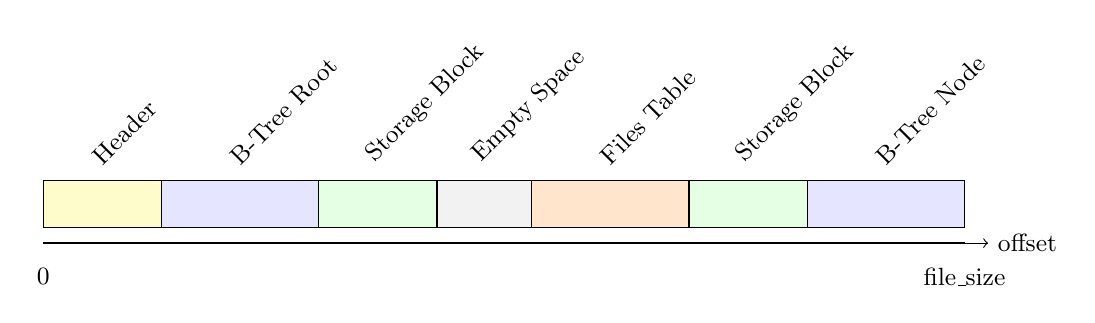
\begin{tikzpicture}[font=\small]

\def\headerW{1.5}
\def\bTreeRootW{2.0}
\def\storageW{1.5}
\def\emptyW{1.2}
\def\filesTableW{2.0}
\def\bTreeNodeW{2.0}

\def\headerX{0}
\def\bTreeRootX{\headerX+\headerW}
\def\storageAX{\bTreeRootX+\bTreeRootW}
\def\emptyX{\storageAX+\storageW}
\def\filesTableX{\emptyX+\emptyW}
\def\storageBX{\filesTableX+\filesTableW}
\def\bTreeNodeX{\storageBX+\storageW}

\pgfmathsetmacro{\totalW}{\headerX+\headerW+\bTreeRootW+\storageW+\emptyW+\filesTableW+\storageW+\bTreeNodeW}
\def\blockH{0.6}

\draw[thick] (0,-0.2) -- (\totalW,-0.2);
\draw[->] (\totalW,-0.2) -- (\totalW+0.3,-0.2) node[right] {offset};

\draw[fill=yellow!20] (\headerX,0) rectangle (\headerX+\headerW,\blockH);
\draw[fill=blue!10] (\bTreeRootX,0) rectangle (\bTreeRootX+\bTreeRootW,\blockH);
\draw[fill=green!10] (\storageAX,0) rectangle (\storageAX+\storageW,\blockH);
\draw[fill=gray!10] (\emptyX,0) rectangle (\emptyX+\emptyW,\blockH);
\draw[fill=orange!20] (\filesTableX,0) rectangle (\filesTableX+\filesTableW,\blockH);
\draw[fill=green!10] (\storageBX,0) rectangle (\storageBX+\storageW,\blockH);
\draw[fill=blue!10] (\bTreeNodeX,0) rectangle (\bTreeNodeX+\bTreeNodeW,\blockH);

\node[anchor=south west, rotate=45] at (\headerX+\headerW/2, \blockH) {Header};
\node[anchor=south west, rotate=45] at (\bTreeRootX+\bTreeRootW/2, \blockH) {B‑Tree Root};
\node[anchor=south west, rotate=45] at (\storageAX+\storageW/2, \blockH) {Storage Block};
\node[anchor=south west, rotate=45] at (\emptyX+\emptyW/2, \blockH) {Empty Space};
\node[anchor=south west, rotate=45] at (\filesTableX+\filesTableW/2, \blockH) {Files Table};
\node[anchor=south west, rotate=45] at (\storageBX+\storageW/2, \blockH) {Storage Block};
\node[anchor=south west, rotate=45] at (\bTreeNodeX+\bTreeNodeW/2, \blockH) {B‑Tree Node};

\node[below] at (0,-0.4) {0};
\node[below] at (\totalW,-0.4) {file\_size};

\end{tikzpicture}
\caption{Расположение структур внутри файла-контейнера. В начале расположен заголовок, а далее структуры расположены в произвольном порядке, который создается за счёт аллокатора.}
\label{fig:file-layout}
\end{figure}

Файл-контейнер (физический файл в файловой системе) представляет собой бинарный файл, в котором содержатся следующие структуры: заголовок (конфигурация библиотеки, адрес узла B-дерева, список логических файлов), узлы B-дерева и сжатые блоки данных. Узлы B-дерева и сжатые блоки данных расположены вперемешку после заголовка, что возможно благодаря использованию аллокатора блоков в файле. Такой файл-контейнер полностью самодостаточен и легко подвергается переносу с одной машины на другую, так как содержит в себе всю необходимую для работы библиотеки информацию.

\subsection{Блочное сжатие и управление внутренней фрагментацией}

Для поддержки эффективного произвольного доступа логический файл делится на блоки произвольного размера, каждый из которых сжимается независимо друг от друга. Так как библиотека должна поддерживать не только операции read/write, но и insert/erase (вставка и удаление), которые могут смещать существующие данные, простое деление файла на блоки фиксированного размера не сработает (при операциях вставки и удаления пришлось бы заново распаковывать все последующие блоки, заново производить разделение и снова сжимать). Поэтому было решено поддерживать блоки произвольного размера, что позволяет реализовать операции вставки и удаления эффективно.

Однако блоки произвольного размера привносят проблему внутренней фрагментации: блоки могут быть слишком маленькие (из-за чего их будет много, а значит потребуется более глубокое B-дерево и данные будут сжиматься хуже), либо слишком большие (из-за чего придется распаковывать большие блоки даже для самых маленьких операций, затрагивающих всего несколько байт). Это существенно замедляет работу библиотеки и делает ее более затратной по памяти.

Для решения проблемы внутренней фрагментации были введены три параметра конфигурации: 
\begin{itemize}
    \item \texttt{block\_size} --- целевой размер блока, который используется при создании новых блоков;
    \item \texttt{block\_size\_\_minimum} --- минимальный размер блока, ниже которого уходить нельзя (если появляется блок с таким размером, то производится попытка склеить его с соседним блоком);
    \item \texttt{block\_size\_\_maximum} --- максимальный размер блока, выше которого уходить нельзя (если появляется блок с таким размером, он делится на несколько блоков).
\end{itemize}

Эти правила применяются во время операций модификации \texttt{write/insert/erase} по отношению к тем блокам, которые затрагиваются операцией. Например если insert вставляет данные внутрь существующего блока, то если суммарный размер не превосходит \texttt{block\_size\_\_maximum}, то новых блоков не создается, а только увеличивается существующий блок. Если же размер блока превзойдет \texttt{block\_size\_\_maximum}, то он делится на несколько блоков (для этого используется \texttt{block\_size}) валидного размера.

\subsection{Индексация блоков: B-дерево} \label{btree}

Для каждой операции чтения или записи необходимо сначала понять какие блоки содержат нужные нам данные. В случае, если бы не было бы требования поддерживать операции вставки и удаления, то размеры блоков можно было бы сделать фиксированными, и тогда понять какие блоки нам нужны было бы нетрудно (чтобы получить номер блока по позиции в логическом файле нужно было бы просто поделить нацело его на размер блока). И тогда все, что нам бы оставалось сделать это сохранить в файле список физических адресов сжатых блоков внутри файла.

Однако в нашем случае блоки могут быть произвольного размера, и поэтому для индексации блоков внутри логических файлов используется \textbf{B-дерево} --- древовидная структура данных ключ-значение, оптимизированная под хранение своих узлов на диске (а не в оперативной памяти). Так как библиотека подразумевает работу с большими данными, структура данных для индексации так же может быть большой, и потенциально она может не вмещаться полностью в оперативную память. B-дерево отлично подходит для данной задачи, так как для работы с ним нам не нужно хранить его в оперативной памяти, а можно только подгружать нужные узлы с диска, когда это требуется. Узлы B-дерева могут быть сколь угодно большими (это настраиваемый параметр), что позволяет сделать их размером со страницу блочного устройства, тем самым не замедлив операцию чтения одного узла, но сильно уменьшив глубину дерева, а значит и количество узлов, которые нужно прочитать при запросах к B-дереву. Так же B-дерево является сбалансированным по своему устройству, что гарантирует логарифмическую сложность операций к нему.

В B-дереве в качестве ключа используется пара \texttt{(hash, pos)}, где \texttt{hash} --- хэш от имени логического файла, а \texttt{pos} --- позиция внутри логического файла. В качестве значения же --- \texttt{(addr, size)}, где \texttt{addr} --- адрес блока внутри файла-контейнера и \texttt{size} --- размер блока. Таким образом для обслуживания всех логических файлов используется одно B-дерево.

% TODO: возможно разбить на подподразделы

Для поддержки операций вставки и удаления необходимо иметь возможность смещать существующие данные. Использование древовидной структуры данных (B-дерево) для индексации блоков позволяет реализовать такую операцию достаточно эффективно (амортизированная логарифмическая сложность). Чтобы понять как, сначала рассмотрим наивную реализацию: чтобы сместить ключи в каком-то промежутке на какое-то смещение, мы рекурсивно проходимся по B-дереву, доходя до всех узлов, в которых содержатся ключи из промежутка, и обновляем эти ключи. Проблема в том, что в худшем случае нам нужно будет обратится вообще ко всем узлам B-дерева.

Чтобы реализовать эту операцию эффективно были реализованы отложенные операции. Идея заключается в том, что в каждом узле для каждого ребенка хранится смещение, которое означает, что все ключи соответствующего ребенка должны быть смещены на эту величину. Вместо того, чтобы сразу смещать все элементы рекурсивно, мы распространяем смещение лениво (только тогда, когда мы спускаемся в соответствующего ребенка), из-за чего и достигается амортизированная логарифмическая сложность.

\subsection{Многофайловость}

Как уже было замечено, в B-дереве используется составной ключ \texttt{(hash, pos)}. В результате в B-дереве ключи из разных логических файлов лежат последовательно и сгуппированно. Это позволяет поддержать многофайловость без каких-либо дополнительных структур данных, кроме единого B-дерева.

Имена файлов и их размеры хранятся в таблице файлов --- динамическом массиве, который располагается в контейнере и управляется аллокатором блоков аналогично узлам B-дерева и сжатым данным. Адрес таблицы хранится в заголовке контейнера. При добавлении нового файла таблица при необходимости расширяется, что позволяет поддерживать произвольное количество файлов в архиве. Явное хранение размера в таблице упрощает получение этой информации без обхода B-дерева.

\subsection{Кэширование}

Наивная реализация каждой операции над логическим файлом приводит к многократным обращениям к диску и частым операциям сжатия/распаковки. Типичная операция чтения требует последовательного получения адреса корня B-дерева из заголовка, загрузки корневого узла, спуска по дереву до целевого листа (с чтением всех промежуточных узлов), затем чтения сжатого блока данных и его декомпрессии. Операция записи дополнительно включает сжатие модифицированных данных, управление местом в файле-контейнере через аллокатор, обновление адреса в узле B-дерева и, возможно, перебалансировку дерева.

С доступами к диску отчасти справляется страничный кэш операционной системы (\texttt{page cache}), однако операции сжатия и распаковки остаются доминирующими по времени выполнения. Именно они создают основную вычислительную нагрузку при работе с архивом. Для снижения этих накладных расходов в библиотеке реализованы два независимых кэша: кэш узлов B-дерева и кэш распакованных блоков данных. Оба направлены в первую очередь на то, чтобы избежать повторного сжатия и распаковки одних и тех же данных.

\subsubsection{Кэш узлов B-дерева}

Кэш узлов B-дерева хранит в оперативной памяти узлы, которые были недавно загружены с диска. Вытеснение производится по алгоритму \textit{LRU} (Least Recently Used). Для повышения производительности в многопоточном окружении кэш является шардированным: он разбит на несколько независимых кэшей (шардов), каждый из которых защищён отдельным мьютексом. Эффективность кэша определяется тем, что корень B-дерева и узлы верхних уровней посещаются при каждом запросе к индексу. Если размер кэша превышает глубину дерева (а она логарифмически мала относительно объёма данных), эти узлы практически никогда не вытесняются, и большинство операций с индексом обходится без операций с диском.

\subsubsection{Кэш блоков данных}

Кэш блоков данных хранит не сжатые данные, а уже распакованные фрагменты логических файлов. При обращении к некоторому участку логического файла соответствующий сжатый блок читается из контейнера, распаковывается и помещается в кэш. При высокой локальности доступа, когда множество последовательных операций приходятся на одни и те же или соседние блоки, кэш блоков данных позволяет свести распаковку только к первому обращению к блоку. В предельном случае, когда рабочий набор данных полностью помещается в кэш, производительность чтения и записи приближается к работе с несжатыми данными в оперативной памяти: все операции обслуживаются из кэша, а сжатие и распаковка выполняются лишь единожды — при загрузке блока и при его вытеснении. Все последующие операции чтения или записи в пределах этого блока выполняются непосредственно в кэше без обращения к диску и, что важнее, без повторного сжатия или распаковки. Именно за счёт сохранения распакованного состояния достигается главный выигрыш в производительности: затратные вычисления компрессора выполняются только один раз при загрузке блока и ещё раз при его вытеснении, если данные были модифицированы.

Вытеснение блоков из кэша производится по алгоритму \textit{2Q-LRU} (Two-Queue Least Recently Used). В отличие от классического LRU, 2Q-LRU использует две очереди: \textit{in-queue} (FIFO-очередь для новых элементов) и \textit{main-queue} (LRU-очередь для «ветеранов»). Новый блок при первом помещении в кэш попадает в \textit{in-queue}. Если к нему происходит повторное обращение, он перемещается в \textit{main-queue}, где дальнейшее вытеснение происходит уже по LRU. Такой подход защищает кэш от однократных «холостых» запросов: блок, который был прочитан всего один раз, не вытесняет часто используемые данные из основной очереди. При вытеснении блока из кэша изменённые данные сжимаются и записываются обратно в файл-контейнер. Таким образом, в случае попадания в кэш удаётся полностью избежать операций сжатия и распаковки, что критически важно для интерактивной работы с большими объёмами данных.
